% Created 2021-09-07 Tue 22:19
% Intended LaTeX compiler: pdflatex
\documentclass{scrartcl}
\usepackage[utf8]{inputenc}
\usepackage[T1]{fontenc}
\usepackage{fontspec}
\usepackage{graphicx}
\usepackage{grffile}
\usepackage{longtable}
\usepackage{wrapfig}
\usepackage{rotating}
\usepackage[normalem]{ulem}
\usepackage{amsmath}
\usepackage{textcomp}
\usepackage{amssymb}
\usepackage{capt-of}
\usepackage[dvipsnames]{xcolor}
\usepackage[colorlinks=true, linkcolor=Blue, citecolor=BrickRed, urlcolor=PineGreen]{hyperref}
\usepackage{indentfirst}
\setmainfont[Ligatures=TeX]{Alegreya}
\setmonofont[Ligatures=TeX]{Liga SFMono Nerd Font}
\usepackage{chemfig}
\usepackage[version=4]{mhchem}
\usepackage{enumerate}

% features: (acronym underline par-sep table)
\newcommand{\acr}[1]{\protect\textls*[110]{\scshape #1}}
\newcommand{\acrs}{\protect\scalebox{.91}[.84]{\hspace{0.15ex}s}}
\usepackage[normalem]{ulem}
\setlength{\parskip}{\baselineskip}
\setlength{\parindent}{0pt}

\usepackage{longtable}
\usepackage{booktabs}
% end features
\author{Shaurya Singh}
\date{\today}
\title{Ap Chem Summer Assignment \#3}
\colorlet{greenyblue}{blue!70!green}
\colorlet{blueygreen}{blue!40!green}
\providecolor{link}{named}{greenyblue}
\providecolor{cite}{named}{blueygreen}
\hypersetup{
  pdfauthor={Shaurya Singh},
  pdftitle={Ap Chem Summer Assignment \#3},
  pdfkeywords={},
  pdfsubject={},
  pdfcreator={Emacs 28.0.50 (Org mode 9.5)},
  pdflang={English},
  breaklinks=true,
  colorlinks=true,
  linkcolor=,
  urlcolor=link,
  citecolor=cite
}
\urlstyle{same}
\begin{document}

\maketitle

\section{The following reaction was performed, Identify element X.}
\label{sec:org107d6dd}
\begin{align*}
  &\ce{Fe2O_3(s)}+\ce{2X(s)} = \ce{2Fe(s) + X_2O_3(s)}\\
  &79.847g+2x=55.847g+50.982g\\
  &\Rightarrow\ 2x=106.829g-79.847g\\
  &\Rightarrow\ 2x=26.982g\\
\end{align*}

Since the atomic weight of \(\ce{Fe}\) is proportional to the given weight
(\(55.847g\)), the atomic weight of X is equally proportional to the derived
weight (\(26.982g\)). \textbf{Therefore, the element is Aluminium (\(\ce{Al}\)).}

\section{Fill in the blanks to balance the following chemical equations:}
\label{sec:org5fb695a}
\begin{enumerate}[a.]
\item \(\ce{2AgI + Na2S} \rightarrow \ce{Ag2S + 2NaI}\)
\item \(\ce{(NH4)2Cr2O7} \rightarrow \ce{Cr2O3}+\ce{N2}+\ce{4H2O}\)
\item \(\ce{Na3PO4}+\ce{3HCl} \rightarrow \ce{3NaCl}+\ce{H3PO4}\)
\item \(\ce{TiCl4}+\ce{2H2O} \rightarrow \ce{TiO2}+\ce{4HCl}\)
\item \(\ce{Ba3N2}+\ce{6H2O} \rightarrow \ce{3Ba(OH)2}+\ce{2NH3}\)
\item \(\ce{3HNO2} \rightarrow \ce{HNO3}+\ce{2NO}+\ce{H2O}\)
\end{enumerate}

\section{Balance the following equation:}
\label{sec:orgcc89537}
We can multiple \(\ce{NH4OH}\) by 4, and increase NH4 and H2O on the product
side to compensate

\textbf{Balanced equation}:

\(\ce{4NH4OH(aq) + KAl(SO4)2} \cdot \ce{12H2O(s)} = \ce{Al(OH)3(s)} +
\ce{2(NH4)2Cr2O7 + KOH(aq)} + \ce{12H2O(l)}\)

\section{Balance the following equation}
\label{sec:org272fc2c}
We need to increase the number of acetate ions on the right side to match the
ones on the left. We also need to increase the right hand side to match the
number of hydrogen atoms on the left.

\textbf{Balanced equation}:
\(\ce{2Fe(s)}+\ce{6HC2H3O2(aq)}=\ce{2Fe(C2H3O2)3(aq)}+\ce{3H2(g)}\)

\section{How many grams of water vapor can be generated from the combustion of 18.74 g of ethanol \(\ce{C2H6O}\)?}
\label{sec:orgb325ef7}
Balanced reaction:
\(\ce{C2H6O(g) + 3O2(g)} \rightarrow \ce{C2O2(g) + 3H2O(g)}\)

Given: ethanol (\(\ce{C2H6O}\)) =  18.74 g

To be calculated : gms of water vapour (H2O) generated after combustion

\textbf{Calculating how many mol of ethanol we have:}

Molar mass of ethanol = 46.07 g/mol

Mass(g) of ethanol = 18.74g

Mol = Mass in grams(g) / molar mass (g/mol)

\begin{align*}
mol&=18.74/46.07\\
&=.4068\\
\end{align*}

\textbf{Multiply this by the ratio of H2O produced from the combustion of ethanol 3 H2O molecules were produced from 1 C2H6O molecule}
\begin{align*}
\text{mol of H2O}&=\text{mol of C2H6O} * (\text{molecules produced of H2O}/\text{molecules of reactant of C2H6O})\\
&=0.4068mol \times (3/1)\\
&=1.22mol
\end{align*}

\textbf{Convert mol back to grams}

Mass(g) / molar mass(g/mol) = \# of mol

Mass(g) = \# of mol * molar mass(g/mol)

\begin{align*}
\text{Mass of H2O(g)}&=1.22mol * 18.015(g/mol)\\
&= 21.99g
\end{align*}

\textbf{Therefore, we will get 21.99g of water vapor}

\section{How many grams of potassium iodide are necessary to completely react with 20.61g of Mercury (II) chloride}
\label{sec:orga18793d}
Balance the equation:
\(\ce{HgCl2 + 2KI(aq)} \rightarrow \ce{HgI2(s) + 2KCl(aq)}\)

\textbf{Find the molar mass of HgCl and 2KI (g/mol)}

\(\ce{HgCl2} = 200.59 + 2(35.45)\)

\(= 271.49\)

\(\ce{2KI} = 2(39.10 + 126.90)\)

\(= 332\)

\textbf{We calculate the ratio of KI to HgCl2}

Ratio = 2KI/HgCl2

\(= 332/271.49\)

\(= 1.22\)

Multiply this by the amount of HgCl2 used to get the amount of Potassium Iodide
needed

\(20.61 \cdot 1.22 = 25.20g\)

\textbf{Therefore, 25.20g of Potassium Iodide is needed}

\section{A reaction combines 113.484 g of lead (II) nitrate with 45.010 g of sodium hydroxide (NaOH[aq]).}
\label{sec:org3858a5e}
The equation for the reaction is
\(\ce{Pb(NO3)2}+\ce{2NaOH}\rightarrow\ce{Pb(OH)2}+\ce{2NaNO3}\)

The molecules molar mass's are

\(\ce{Pb(OH)2}=241.196 amu\)

\(\ce{Pb(NO3)2}=331.207 amu\)

\(\ce{2NaOH}=79.94 amu\)

\(\ce{2NaNO3}=169.99 amu\)

\begin{enumerate}[a.]
\item We know that \(331.207\) amu of  lead nitrate can react with \(79.94\) amu of sodium
hydroxide. Therefore, \(113.484g\) of lead nitrate will react with
\(\frac{113.484*79.94}{331.207}g\), or \(27.41g\) of sodium hydroxide

Similarly, we know that \(331.207\) amu of  lead nitrate can produce \(241.196\) amu of lead
hydroxide. Therefore, \(113.484g\) of lead nitrate will produce
\(\frac{113.484*241.196}{331.207}g\), or \(82.643g\) of lead hydroxide
\item Lead(II) nitrate is the limiting reactant since it produces the least amount
of Lead Hydroxide.
\item There is \(45.010-27.408=17.602\) grams of the excess reactant left over.
\item From the above we get an experimental yield of \(80.02\) percent. We know the
limiting reactant gives us a theoretical yield of \(82.463\) percent.
Therefore, the percent yield is    \((\frac{80.02}{82.463}\times100=97.04)\), or 97.04\%
\end{enumerate}

\section{A reaction combines 64.81 grams of silver nitrate with 92.67 grams of potassium bromide}
\label{sec:orgc1ae34f}
\textbf{The equation for the reaction is already balanced:}
\(\ce{AgNO3}+\ce{KBr}\rightarrow\ce{AgBr}+\ce{KNO3}\)

\begin{enumerate}[a.]
\item Calculate the atomic weight of the reactants and \(\ce{AgBr}\):

\(\ce{AgNO3} = 169.872g\)

\(\ce{Kbr} = 119.002g\)

\(\ce{AgBr} = 187.772g\)

Now we can calculate how much \(\ce{AgBr}\) each reactant made

\(\ce{AgNO3}\): \(\frac{64.81\times187.772g}{169.872}=71.64g\)

\(\ce{KBr}\): \(\frac{92.67\times187.772g}{119.002}=146.2g\)

Therefore,   \(71.64g\) of \(\ce{AgBr}\) will be made, since \(\ce{AgNO3}\) is the limiting reactant.

\item \(\ce{AgNO3}\) is the limiting reactant since it produces the least amount of
\(\ce{AgBr}\). Therefore the excessive reactant is  \(\ce{Kbr}\) since it
produced the most amount of AgBr
\item To calculate how much excessive reactant is left over, we can use the
theoretical yield and find the mass of the excessive reactant used:

\(\frac{71.64\times119.002g}{187.772}=45.40\), or \(45.40g\) of KBr
\item In order to find the percent yeild, divide the actual yield by the
theoretical yield, then multiply by 100:

\(\frac{14.77g}{71.64g}\times100=20.62\), or \(20.62\) percent.
\end{enumerate}

\section{The moleculer weight of an insecticide, dibromoethane, is 187.9. Its molecular formula is \(\ce{C2H4Br2}\), What percent by mass of bromine does dibromoethane contain?}
\label{sec:org27b60ea}
\textbf{We must calculate the atomic weight for each element}
\begin{align*}
&\ce{C} = 12.011\\
&\ce{H} = 1.008\\
&\ce{Br} = 79.90
\end{align*}

Since the formula is  \(\ce{C2H4Br2}\), we can substitute the atomic weights in
place of the elements
\begin{align*}
&= 2(\ce{C}) + 4(\ce{H}) + 2(\ce{Br})\\
&= 2(12.011) + 4(1.008) + 2(79.90)\\
&= 24.022 + 4.032 + 159.8\\
&= 187.9
\end{align*}

Finally, we need to divide the amount of bromine by the total amount in order to
find the percent by mass of bromine in \(\ce{C2H4Br2}\)
\begin{align*}
&= \frac{159.8}{187.9}\\
&=.8505
\end{align*}

\textbf{Therefore, dibromoethane contains 85.05\% by mass of bromine.}

\section{A given sample of xenon fluoride contains molecules of a single type of \(\ce{XeFn}\), where n is some whole number.}
\label{sec:org533ba7d}
First, we need to calculate how many moles of xenon fluoride there are, and
calculate its weight

\begin{align*}
moles&=9.03*10^{20}/6.022*10^{23}\\
&= 1.5*10^-3\\
&= 0.31g
\end{align*}

Now, we can calculate for \(n\)

\begin{align*}
&= 0.31/131+19n\\
&= 186.5 + 23.5n = 310\\
&n = 4
\end{align*}

\textbf{Therefore its formula is \(\ce{XeF4}\)}

\section{A 6.32 g sample of potassium chlorate was decomposed according to the following equation, how many moles of \(\ce{O2}\) were formed?}
\label{sec:org2ee6d32}
We are given the following formula for the reaction:

\(\ce{2KCIO3} \rightarrow\ce{2KCL}+ \ce{3O2}\)

We have the following values:
\begin{align*}
&k = 39.0983g\\
&Cl = 35.45g\\
&O = 16.00g
\end{align*}

From there we can calculate the total molar mass
\begin{align*}
&39.0983 + 35.45 + 3*16 = 122.55g
\end{align*}

Now, by performing dimensional analysis we get the following equation to convert
grams of potassium chlorate to moles of oxygen
\begin{align*}
  \text{mol}&=\frac{6.32g}{1}\times\frac{1mol}{122.548g}\times\frac{3}{2}\\
  &=\frac{6.32g*3}{(122.648*2)}\\
  &=7.74*10^{-2}\\
\end{align*}

\textbf{Therefore, \(7.74*10^{-2}\) moles of \(\ce{O2}\) is formed}

\section{What is the coefficient in front of water, when it is produced from the reaction of hydrochloric acid with calcium hydroxide? Calcium chloride is the other product.}
\label{sec:org3ce3e22}
The balanced equation is
\(\ce{Ca(OH)2 + 2HCl}=\ce{CaCl2 + 2H2O}\)

\textbf{Therefore the coeffecient of water (\(\ce{H2O}\)) is 2}

\section{What is the subscript of aluminum in the formula of aluminum phosphate?}
\label{sec:orga9b8d0e}
\textbf{Aluminum has a subscript of \(1\) in \(\ce{AlPO4}\)}

\section{The reaction of 11.9 g of \(\ce{CHCl3}\) with excess chlorine produced 12.6 g of \(\ce{CCl4}\), carbon tetrachloride, what is the percent yield?}
\label{sec:orgbed1fad}
The equation for the reaction is
\(\ce{2CHCl3 + 2Cl2}=\ce{2CCl4 + 2HCl}\)

We need to calculate the theoretical yield of this reaction. To do that, we need
to calculate the atomic weight of \(\ce{CHCl3}\) and \(\ce{CCl4}\).

\(\ce{ChCl3}\): \(119.378g\)

\(\ce{CCL4}\): \(153.823g\)

Now we can find the theoretical yield:
\begin{align*}
  &=\frac{11.9g}{1}\times\frac{1mol}{119.378g}\times\frac{2}{2}\times\frac{153.823g}{1}\\
  &=\frac{11.9*2*153.823g}{(119.378*2)}\\
  &=15.3g\\
\end{align*}

To find the percent yield, divide the experimental yield by the theoretical
yield, then multiply by 100
\begin{align*}
  &=\frac{12.6g}{15.3g}\times100\\
  &=82.4\\
\end{align*}

\textbf{Therefore the percent yield is 82.4\%}

\section{What mass of \(\ce{CCl}\) 4 is formed by the reaction of 8.00 g of methane with an excess of chlorine?}
\label{sec:org1fdec8d}
The given equation is already balanced. The question is asking us to calculate
the theoretical yield

We need to calculate the atomic weight of \(\ce{CCl4}\) and \(\ce{CH4}\)

\(\ce{CCl4}\): \(153.823g\)

\(\ce{CH4}\): \(16.043g\)

We already know \(\ce{CH4}\) is the limiting reactant. Using dimensional analysis, we can calculate the theoretical yield
\begin{align*}
&=\frac{8.00g}{1}\times\frac{1}{16.043g}\times \frac{1}{1}\times \frac{153.823g}{1}\\
&=\frac{8 \times 153.823g}{16.043}\\
&=76.7g\\
\end{align*}

\textbf{Therefore, \(76.72g\) of \(\ce{CCl4}\) is formed by the reaction.}

\section{A reaction occurs between sodium carbonate and hydrochloric acid producing sodium chloride, carbon dioxide, and water. Write the balanced chemical equation for the reaction.}
\label{sec:orgfd6bfaa}
The equation will be sodium carbonate + hydrohloric acid = sodium chloride +
carbon doxide + water. In correct notation this is written as:

\begin{align*}
&\ce{Na2CO3 + HCl}\rightarrow\ce{NaCl + CO2 + H2O}
\end{align*}

Balanced, this equation is
\begin{align*}
&\ce{Na2CO3 + 2HCl}\rightarrow\ce{2NaCl + CO2 + H2O}
\end{align*}

\section{Classify the type of reaction from the five major type of reactions you learned in your first year chemistry course and write word equations. If necessary, balance.}
\label{sec:org069f7ad}
\begin{enumerate}[a.]
\item The word equation is \textbf{Sodium Hydroxide + Potassium Nitrate \(\rightarrow\) Sodium
Nitrate + Potassium Hydroxide}. This equation is already balanced, and is a
double replacement reaction since the two positive ions switched the negative
ions they are bonded with.
\item The balanced reaction is \(\ce{CH4 + 2O2}\rightarrow\ce{CO2 + 2H2O}\). The word
equation for this is \textbf{Methane + Oxygen Gas \(\rightarrow\) Carbon Dioxide + Water}.
This is a combustion reaction since \(\ce{CH4}\) reacted with oxygen gas.
\item The balanced reaction is \(\ce{Fe + 3NaBr}\rightarrow\ce{FeBr3 + 3Na}\). The word
equation for this is \textbf{Iron + Sodium Bromide \(\rightarrow\) Iron(III)Bromide +
Sodium}. This is a single replacement reaction since the negative ion in the
reactants switches the positive ion its bonded with.
\item The word equation is \textbf{Calcium Sulfate + Magnesium Hydroxide \(\rightarrow\)
Calcium Hydroxide + Magnesium Sulfate}. This equation is already balanced, and
is a double replacement reaction since the two positive ions switched the
negative ions they are bonded with.
\item The word equation is \textbf{Ammonium Hydroxide + Hydrobromic Acid \(\rightarrow\)
Water + Ammonium Bromide}. This equation is already balanced, and is a double
replacement reaction since the two positive ions switched the negative ions
they are bonded with.
\item The word equation is \textbf{Lead + Oxygen Gas \(\rightarrow\) Lead(IV)Hydroxide}. This
equation is already balanced, and is a synthesis reaction since the two
reactants combined to form one product.
\item The word equation is \textbf{Sodium Carbonate \(\rightarrow\) Sodium Oxide + Carbon
Dioxide}. This equation is already balanced, and is a decomposition reaction
since a compound (in this case the reactant) breaks down
\end{enumerate}

\section{Now try these reaction types, Rewrite as a balanced equation with the products predicted}
\label{sec:orgbd17dff}
\begin{enumerate}[a.]
\item \(\ce{Ba(OH)2}\rightarrow\ce{BaO + H2O}\)
\item \(\ce{Na2CO3}\rightarrow\ce{Na2O + CO2}\)
\item \(\ce{2LiClO3}\rightarrow\ce{2LiCl + 3O2}\)
\item \(\ce{2Al2O3}\rightarrow\ce{4Al2 + 3O2}\)
\item \(\ce{H2SO4}\rightarrow\ce{H2O + SO3}\)
\end{enumerate}

\section{Now try these reaction types, Rewrite as a balanced equation with the products predicted}
\label{sec:orgfa30bf4}
\begin{enumerate}[a.]
\item \(\ce{2Mg + O2}\rightarrow\ce{2MgO}\)
\item \(\ce{N2 + 3H2}\rightarrow\ce{2NH3}\)
\item \(\ce{S + O2}\rightarrow\ce{SO2}\)
\item \(\ce{CaO + H2O}\rightarrow\ce{Ca(OH)2}\)
\end{enumerate}

\section{Attempt to write and predict products the following chemical reactions:}
\label{sec:org270d7a4}
\begin{enumerate}[a.]
\item \(\ce{2H2O2}\rightarrow\ce{2H2O + O2}\)
\item \(\ce{Ba(OH)2 + CuSO4}\rightarrow\ce{Cu(OH)2 + BaSO4}\)
\item \(\ce{Al + 3AgNO3}\rightarrow\ce{Al(NO3)3 + + 3Ag}\)
\item \(\ce{Cl2 + 2NaBr}\rightarrow\ce{Br2 + 2NaCl}\)
\item \(\ce{2C2H6 + 7O2}\rightarrow\ce{4CO2 + 6H2O}\)
\end{enumerate}

\section{Review the next section and the video, then answer the following}
\label{sec:org80269dd}
\subsection{Part A: Using the solubility rules table, classify each of the substances as being soluble or insoluble in water.}
\label{sec:orgb112617}
\begin{enumerate}[a.]
\item \(\ce{KBr}\) = Soluble

Based on the soluble salt rules, bromine anions are
soluble when bonded with a cation that isn't \(\ce{Pb}\), \(\ce{Ag}\),
or \(\ce{Hg2+}\). This means that \(\ce{Kbr}\) is soluble.

\item \(\ce{PbCO3}\) = Insoluble

Since \(\ce{Pb}\) isn't from group 1 and there
aren't any rules for \(\ce{CO3}\), \(\ce{PBCO3}\) is insoluble.

\item \(\ce{BaSO4}\) = Insoluble

Based on the soluble salt rules, when
\(\ce{SO4}\) is bonded with Ba, it makes it insoluble

\item zinc hydroxide = Insoluble

\(\ce{Zn(OH)2}\) is amphateric but it isn't a
strong acid or a strong base, so its insoluble

\item sodium acetate = Soluble

\(\ce{NaCH3COO}\) is soluble since the cation is
from the first group of the periodic table and the anion is the polyatomic
ion acetate, both of whitch are always soluble in a compound

\item silver iodide = Insoluble

\(\ce{AgI}\) is insoluble since the rules of
soluble salts state that when the anion I is in a compound with Ag, then it
is insoluble

\item cadmium (II) sulfide = Insoluble

\(\ce{CdS}\) is insoluble since there is
no rule written about sulfur anions nor cadmium. Cadmium also isn't a group 1
element, making the compound insoluble

\item zinc carbonate = Insoluble

\(\ce{ZNCO3}\) is insoluble since there is no
rule written about carbonate polyatomic anions. Zinc also isn't a group 1
element

\item silver acetate = Soluble

\(\ce{AgC2H3O2}\) is soluble since the compound
countains an acetate  polyatomic anion. The soluble salt rule states that any
compound with acetate should be soluble

\item copper (II) sulfide = Insoluble

\(\ce{CuS}\) is insoluble since neither or
copper nor sulfur is included in the soluble salt rules. Copper also isn't a
group 1 element, so the compound is insoluble

\item \(\ce{Mg3(PO4)2}\) = Insoluble

Phosphate is not mentioned in the soluble
salt rules, and magnesium isn't a group one element, so this compound is
insoluble

\item \(\ce{KOH}\) = Soluble

It is in the list of the 8 strong bases

\item \(\ce{NiCl2}\) = Soluble

The soluble salt rule states that when a compound
contains chlorine as anion, as long as the cation it is bonded to isn't
\(\ce{Pb}\),     \(\ce{Ag}\), or \(\ce{Hg2^{2+}}\) it will be a soluble
compound.

\item \(\ce{NH4OH}\) = Soluble

\(\ce{NH4OH}\) contains \(\ce{NH4}\), and based on
the soluble salt rules, the compound containing it is soluble.

\item \(\ce{Hg2SO4}\) = Insoluble

The soluble salt rules state when sulfate is
bonded with     \(\ce{Hg2}\) in a compound, it renders it insoluble

\item \(\ce{PbI2}\) = Insoluble

The soluble salt rule states that when the anion
iodine is bonded to the cation lead, it will be insoluble
\end{enumerate}

\subsection{Part B: Identify the two new compounds that form if the solutions, as suggested by the following table, were mixed via a double displacement reaction.}
\label{sec:org1ac85cb}

Underlined compounds are precipitates of the reaction
\begin{center}
\begin{tabular}{llll}
\toprule
\uline{\(\ce{AgBr(s)}\),} \(\ce{KNO3(aq)}\) & \uline{\(\ce{Ag2CO3(s)}\)}, \(\ce{NaNO3(aq)}\) & \uline{\(\ce{Ag2S(s)}\),}  \(\ce{Ca(NO3)2(aq)}\) & \uline{\(\ce{AgOH(s)}\)}, \(\ce{NH4NO3(aq)}\)\\
\midrule
\(\ce{BaBr2(aq), KCl(aq)}\) & \(\ce{NaCl(aq)}\), \uline{\(\ce{BaCO3(s)}\)} & \(\ce{CaCl(aq), BaS(aq)}\) & \(\ce{Ba(OH)2(aq), NH4Cl(aq)}\)\\
\midrule
\(\ce{AlBr3(aq), KNO3(aq)}\) & \uline{\(\ce{Al2(CO3)3(s)}\),} \(\ce{NaNO3(aq)}\) & \(\ce{AlBr3(aq)}\), \uline{\(\ce{Al2S3(s)}\)} & \uline{\(\ce{Al(OH)3(aq)}\),} \(\ce{NH4NO3(aq)}\)\\
\midrule
\(\ce{K2SO4(aq), CuBr2(aq)}\) & \uline{\(\ce{CuCO3(s)}\),} \(\ce{NaSO4(aq)}\) & \(\ce{K2SO4(aq)}\), \uline{\(\ce{CuS(s)}\)} & \(\ce{NH4(SO4)2(aq)}\), \uline{\(\ce{Cu(OH)2(s)}\)}\\
\bottomrule
\end{tabular}
\end{center}

\section{Name the following, then draw the Lewis Structure for the following hydrocarbons from their full names.}
\label{sec:orgc4225d2}
\begin{enumerate}
\item \(\ce{CH4}\) - methane

Since the compound contains one carbon atom (meth) and there are sigma bonds
(ane), the name of this compound is methane. From the diagram we can see the
molecular formula is    \(\ce{CH4}\)

\item \(\ce{C3H8}\) - propane

Since the compound has three carbon atoms (prop) and there are sigma bonds
(ane), the name of the compound is propane. With the help of the diagram, we
can see the molecular formula is    \(\ce{C3H8}\)

\item Question 3 is missing from the assignment paper

\item \(\ce{C4H8}\) - 1-butene

Since the compound contains four carbon atoms (but) and a central double bond
(ene), the name of this compound is butene.

\item \(\ce{C4H8}\) - 2-butene
Since the compound contains four carbon atoms (but) and a central double bond
(ene), the name of this compound is butene. The \texttt{2-} denotes that this is an
isonomer of butene (different arrangement than \#4 Q. 22).

\textbf{Draw Lewis Structures for the following}

\item Ethane \(\ce{C2H}\)

Based on the name, there are two carbon atoms and sigma bonds are present.
The lewis diagram would be

\begin{center}
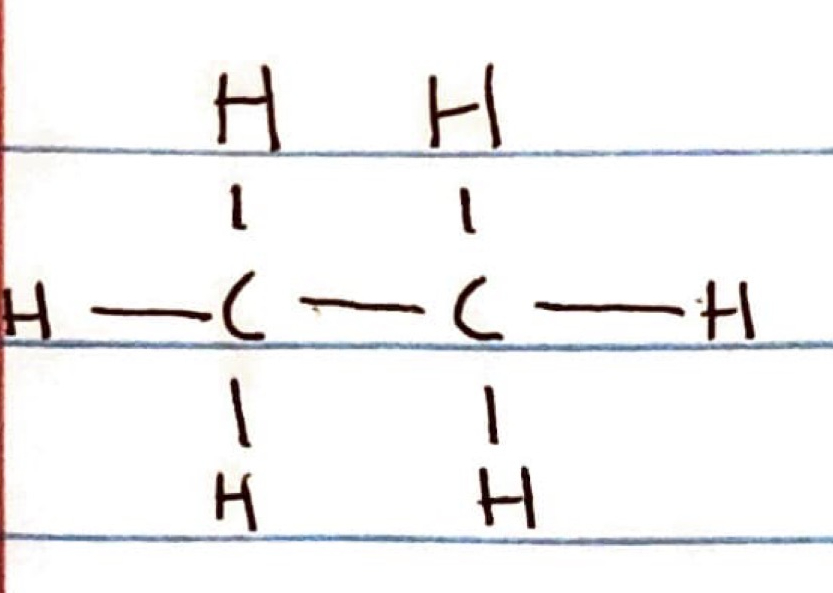
\includegraphics[width=4cm]{./images/6.JPG}
\end{center}

\item Methane \(\ce{CH4}\)

Based on the name, there should be one carbon atom and sigma bonds are
present. The lewis diagram would be

\begin{center}
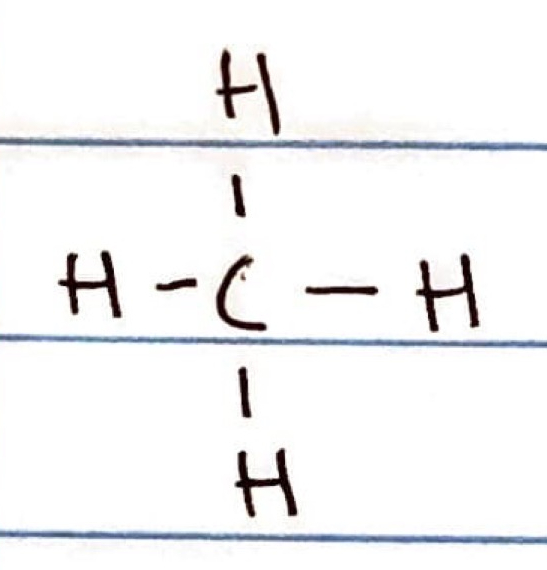
\includegraphics[width=4cm]{./images/7.JPG}
\end{center}

\item Propyne \(\ce{C3H4}\)

Based on the name, there shold be three carbon atoms and a triple bond. The
lewis diagram woudl be

\begin{center}
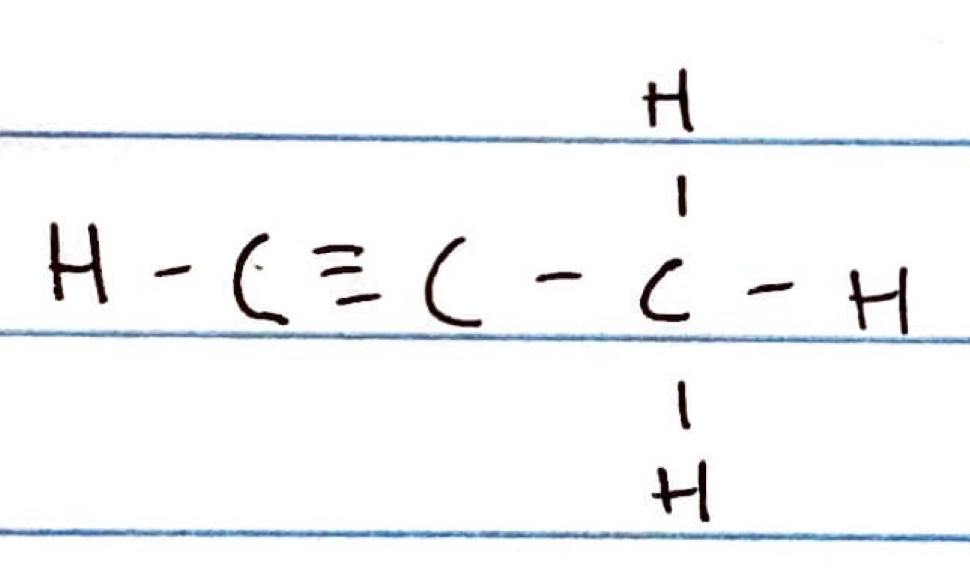
\includegraphics[width=5cm]{./images/8.JPG}
\end{center}

\item 2 \(\cdot\) Butene \(\ce{C4H8}\)

Based on the name, there shuold be four carbon atoms and a double bond. The 2
in front signifies this is an isomer of butene. It's lewis diagram would be

\begin{center}
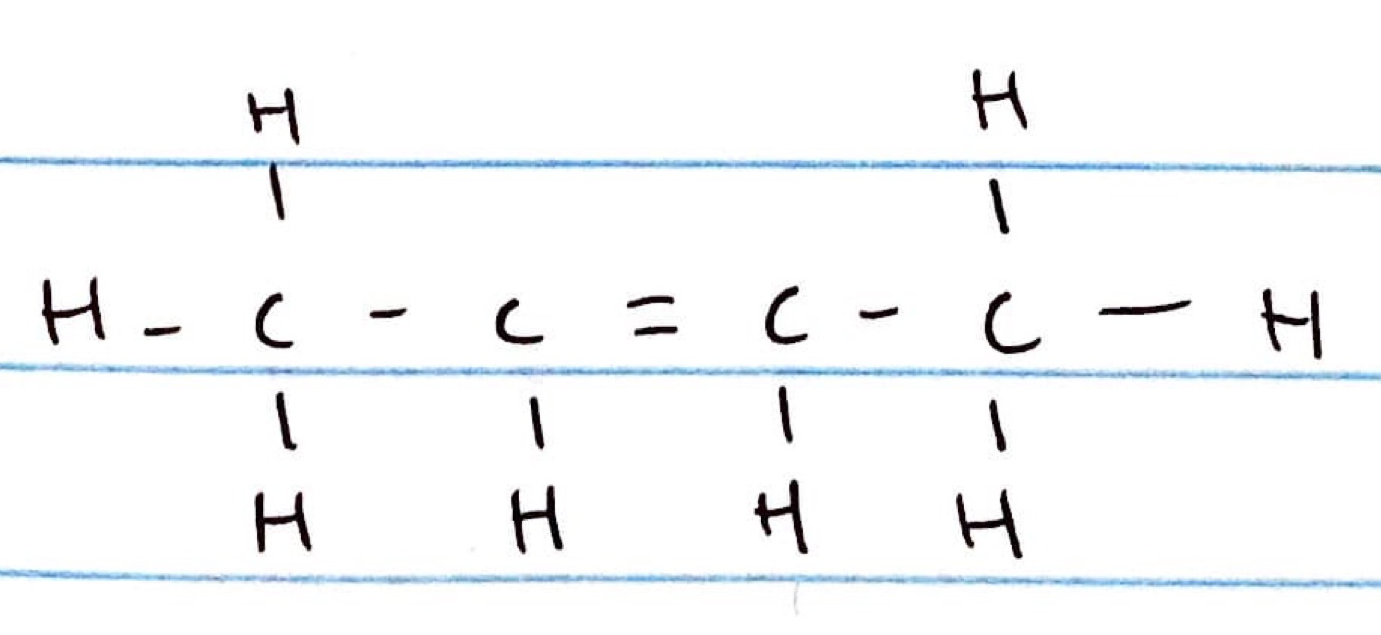
\includegraphics[width=6cm]{./images/9.JPG}
\end{center}
\end{enumerate}
\end{document}
